
%%% Local Variables:
%%% mode: latex
%%% TeX-master: t
%%% End:

\chapter{资源管理软件栈}
\label{chap:prm}

%% 数据中心管理软件要做这些事情
%A datacenter management system brings the benefits of high availability, high
%reliability, high utilization and fast deployment and so on.
%% 它的基本构成是隔离与封装环境,当前使用虚拟化与容器实现
%An essential building block of such management systems is resource isolation and
%encapsulation, which now primarily adopts software based approaches such as
%virtualization and container.
%% 但软件方法没有足够的性能隔离
%However, software approaches are insufficient
%for performance isolation due to the interference on low-level hardware resources
%(e.g., shared cache, memory bandwidth).
%% 因此需要硬件支持
%Thus, to address this issue,
%recently hardware isolation has been proposed and proven to be promising.

数据中心对其管理系统提出了高可用、高可靠、高利用率以及快速部署等需求,
资源隔离与封装是实现以上需求的必要条件。
当前数据中心管理系统大都基于虚拟化、容器等软件技术实现资源隔离与封装。
然而受到底层硬件层次(如处理器末级缓存、内存控制器等)资源竞争与干扰的影响,
这些软件方法无法实现性能隔离,需要在硬件上提供资源隔离机制。

%% 软硬件是交替促进发展的,本章讨论硬件隔离机制如何影响软件的改变,
%% 具体来说本文所提出的PARD体系结构对上层管理软件提出的需求,
%% 包括Hypervisor、操作系统及上层管理软件。
%Since the hardware and the system software always evolve mutually, in this paper
%we discuss how hardware isolation influences system software, including
%Hypervisor, operating system kernel and cluster management system.
%Specifically, we will outline how to modify OpenStack, a popular
%cloud computing platform, to be aware of servers with hardware isolation
%and further take the advantages of hardware isolation.

计算机的软硬需要协同工作,本章主要讨论硬件提供更多资源管理机制后,
对应的系统软件栈(\emph{e.g.} Hypervisor,操作系统,数据中心管理系统)
需要如何适应这种变化。
具体来说,即如何在PARD体系结构下设计系统软件栈,以实现高效的数据中心管理。
本章内容安排如下:
首先介绍数据中心软件栈背景,并对其需求进行分析;
然后分别以Mesos和IPMI为例,介绍节点间与节点内资源管理系统的架构;
之后介绍基于PARD体系结构的数据中心软件栈设计,
包括节点内与节点间(数据中心)2部分,
并具体讨论将PARD体系结构集成到Mesos系统中所需要解决的问题与挑战。

%实现高效资源管理需要软硬件协同设计。
%PARD体系结构已经实现将硬件资源信息暴露给上层软件,
%并提供可编程接口给软件访问,本章主要讨论在PARD这样的硬件架构平台上,
%如何设计软件栈以实现高效的资源管理。

%则一般都会影响甚至重构整个软件栈:最底层的控制平面驱动层,负责直接访问控制平面,这一层可以部署在操作系统、Hypervisor或者一个轻量级的操作系统内核;在驱动层上面为监控管理层,主要负责集中存储收集到的各个控制平面的统计数据,并将多个控制平面关联分析,进行资源分配管理的决策;更上层是用户编程接口层,主要负责提供对控制平面统一的抽象编程接口以及对统一、决策功能的抽象编程接口;最上层则是数据中心管理软件层,主要负责收集几个计算机节点的资源信息,进行全局作业调度与资源管理,以实现在保障关键应用服务质量的前提下达到全局资源利用率最优化。
%因此,从单个计算机节点角度出发,在硬件支持资源管理的基础上,软件栈的设计与实现需要研究上述驱动层、监控管理层与用户接口层的设计与实现,降低软件栈的设计复杂度与运行开销,研究针对不同资源的优化管理策略。同时研究在这种新体系结构下对软件虚拟化技术的影响。
%
%PARD体系结构在硬件上有2方面的改变:一是一部分资源管理功能放到了硬件控制器上;二是将更多的硬件资源信息暴露给软件。计算机底层硬件功能的改变会对上层软件栈产生影响。

\section{背景}

管理大规模数据中心是大型互联网公司运维工作的基本任务,在过去的十几年中,
这些公司开发了不同的管理系统来完成这一任务,
如:Google的Omega\cite{Schwarzkopf_omega_2013}、Borg\cite{borg:2015}、
Kubernetes\cite{Kubernetes},Microsoft的Apollo \cite{Apollo}、Cosmos \cite{Cosmos},
Facebook的Aurora\cite{Aurora},国内百度的Matrix以及阿里的伏羲\cite{Fuxi}。
其他一些开源系统如OpenStack\cite{OpenStack}、Apache Mesos\cite{Hindman:2011:Mesos}、
YARN\cite{YARN}被广泛的应用在工业界。

除提供高可用、高可靠、快速部署等基本管理功能外,
这些数据中心管理系统的另一个重要目标是提高数据中心的资源利用率:
通过应用调度将数据中心百万量级的应用混合运行在十万量级到服务器上,
使用资源共享的方式充分利用服务器资源。
通常情况下,一台物理服务器上会运行多个具有不同资源与服务质量需求的应用。

%However, such workload colocation causes contention over shared hardware and software
%resources such as last level cache (LLC), network bandwidth and kernel buffers, thereby
%resulting in unpredictable performance variation that degrades QoS of
%latency-critical workloads.
%In order to guarantee these workloads' QoS in shared environments,
%current management systems primarily adopt software based resource
%isolation mechanisms, \emph{e.g.}, virtual machine, container and
%control group (cgroup) \cite{cgroup}, due to the lack of hardware supported isolation.
%
%Software based isolation is effective to a certain extend for resource allocation
%and protection but is insufficient for performance isolation, especially due to
%contention over hardware resources.
%
%For example, with more than 10 years of
%experience in operating Borg in Google's production environments, Borg developers
%found that after using a Linux cgroup-based resource container, low-level
%hardware interference still happens \cite{borg:2015}.
%Thus, in Dick Sites' recent talk \cite{Dick:2015}, he argued that better hardware
%support isolation is needed.
正如本文前几章所分析的,多个应用在共享软硬件资源上竞争会对应用造成不可预测的性能下降,
特别是延迟敏感型应用,这种性能下降更为明显。
为了保障在共享环境下关键应用的服务质量,
当前的数据中心管理系统通常会使用软件方法来实现应用之间的隔离,
如虚拟化、容器和cgroup。
虽然软件隔离方案能够很好的实现资源分配与保护,
但它不足以提供有效的性能隔离,特别是由硬件层次上资源竞争所造成的性能干扰。
以Google数据中心为例,即使经过10多年生产环境的运行与优化,
基于cgroup实现软件隔离的Borg系统仍然无法解决硬件层次所带来的干扰\cite{borg:2015}。
因此,正如Dick Sites在其报告\cite{Dick:2015}中所提出,
硬件支持隔离对于数据中心服务器是必不可少的。

本文所提出的PARD体系结构正是这样一种支持硬件隔离的服务器体系结构,
它能够实现全硬件支持虚拟化(第\ref{chap:labeladdrspace}章),
在无需软件Hypervisor的支持下,即可将一台物理服务器划分为多个相互隔离的子机器(逻辑域),
在逻辑域内可以像虚拟机一样运行未修改的操作系统与应用。
同时PARD还提供了以逻辑域为粒度的区分化服务,
通过可编程的硬件资源管理机制实现逻辑域之间的资源划分与性能隔离
(第\ref{chap:hwresman}章)。
基于模拟器的实验结果表明,PARD能够在硬件上实现有效的资源与性能隔离,
平衡应用服务质量与服务器资源利用率。

%To address this issue, we recently proposed a new computer architecture PARD
%(Programmable Architecture for Resourcing-on-Demand) \cite{Ma:2015:PARD}, which
%supports hardware isolation. Specifically, a PARD server is able to provide fully hardware supported
%virtualization without software hypervisors. Thus the server is
%physically partitioned into multiple submachines that can run unmodified OS.
%The PARD server also supports differentiated service (DiffServ) for these submachines,
%which means that each submachine is assigned a priority for performance isolation
%in light of its QoS requirement. Preliminary results on
%a GEM5 \cite{binkert_gem5_2011} based full-system
%cycle accurate simulator and an FPGA-based ongoing PARD server prototype
%further show that hardware isolation is feasible.

%Historically, the hardware and the system software always evolve mutually, such as
%interrupt and time-sharing, memory management unit (MMU) and virtual memory.
%Since recent efforts suggests that the trend of hardware isolation is promising,
%consequent questions arise: \textbf{what is the impact of hardware isolation on system
%software? What's next for system software?}

从计算机发展的历史来看,硬件与系统软件总是总是在相互促进发展的,
如硬件中断机制的出现使得系统软件发展出分时系统、MMU硬件的出现促成了虚拟内存机制。
本文所提出的PARD体系结构,以及其他一些硬件隔离技术的出现\cite{intel-rdt},
势必也会对未来系统软件的设计产生影响。

本章主要讨论如何将PARD服务器集成到现有数据中心管理系统,
并利用其提供的资源管理特性(表\ref{tab:pard-features})实现高效的数据中心管理。
PARD服务器与传统服务器主要的区别在于其提供了细粒度的资源管理、实时的性能监控、
硬件支持的虚拟化与性能隔离,因此更适合于短时多变的作业;
而长期运行,且负载稳定的应用可以通过软件管理的方式在传统服务器中运行。
因此,传统服务器与PARD服务器将混合共存于数据中心,由数据中心管理系统进行统一管理,
为不同类型的应用提供服务。
为实现以上架构,需要考虑2个问题:
1)如何设计节点内资源管理,使其充分发挥PARD体系结构提供的硬件支持;
2)如何修改数据中心管理系统,使其能够支持PARD体系结构。
为解决以上2个问题,本节后续内容将对数据中心管理系统与节点内资源管理架构进行简要介绍。

\begin{table}[hb]
  \centering
  \begin{minipage}[t]{0.7\linewidth}
  \caption{PARD服务器与传统服务器特性对比}
  \label{tab:pard-features}
  \begin{tabular}{rp{0.3\textwidth}<{\centering}p{0.3\textwidth}<{\centering}}
    \toprule[1.5pt]
                             & \textbf{传统服务器} & \textbf{PARD服务器} \\
    \midrule[1pt]
      \emph{Virtualization}  & SW Supported        & HW Supported        \\
      \emph{Perf. Isolation} & Unsupported         & HW Surpported       \\
      \emph{Monitoring}      & High overhead       & Realtime            \\
      \emph{Perf. Adaption}  & Coarse-grained      & Fine-grained        \\
    \bottomrule[1.5pt]
  \end{tabular}
  \end{minipage}
\end{table}


\subsection{数据中心管理系统}

\begin{figure}[tb]
  \centering
  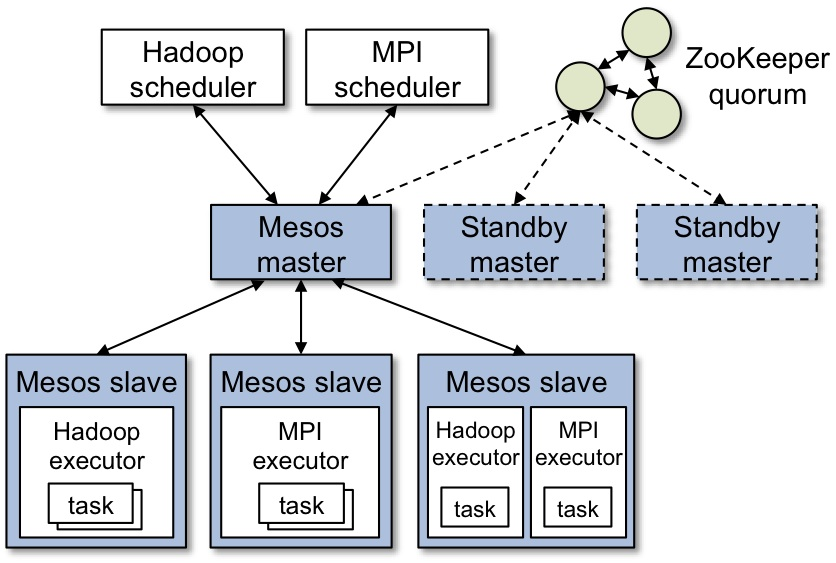
\includegraphics[width=\textwidth]{swstk/mesos-arch}
  \caption{Mesos系统架构}
  \label{fig:mesos-arch}
\end{figure}

如上文所述,数据中心管理系统需要为数据中心提供高可用、高可靠、高利用率以及快速部署支持。
以Apache Mesos\cite{Hindman:2011:Mesos}为例,其架构如图\ref{fig:mesos-arch}所示,
它通过集中式的master节点控制运行在服务器内的slave守护进程实现数据中心资源管理。
master负责管理所有的资源,当slave注册到Mesos集群时,将其提供的资源发送到master进行统一管理,
这些资源主要指CPU、内存、磁盘,除此之外还包括其他用户自定义类型的资源,
以资源列表的形式发送给master,如:

\textit{<slave ID, resource1:amount1, resource2:amount2, ...>}

Mesos为用户提供framework抽象,主要包含2个部分:调度器(scheduler)与执行器(executor)。
其中调度器与master节点交互并获取资源,执行器在slave节点上运行,执行由调度器发送的任务(task)。
master根据用户设定的策略为每个framework分配资源,例如公平划分(fair sharing)或基于优先级的策略(strict priority)。
当master决定分配多少资源给framework后,将资源列表发送到framework的调度器,
调度器从中选择所需的资源,并将调度执行的任务描述发送给master,由其分发到对应的slave节点执行。

%\textbf{Mesos如何实现高可用、高可靠、高利用率以及快速部署?}
Mesos提供了跨节点的细粒度资源管理与作业调度,如图\ref{fig:mesos-arch}所示,
通过基于进程或容器的快速应用部署,将不同资源需要的应用调度到同一个节点,实现高资源利用率。
Mesos在ZooKeeper的辅助下,通过多master选举的方式实现master节点的高可用,
对于其他的组件(如调度器与执行器),
Mesos也提供了相应的方案以实现其高可用\cite{mesos-high-available-framework}。
一些基于Mesos的开源系统,如Marathon\cite{marathon}、Aurora\cite{Aurora}等,
在Mesos功能的基础上,实现了应用自动扩容与出错重启,满足了高可用与高可靠需求。


\subsection{节点内资源管理架构}

数据中心管理系统所提供的功能需要节点内提供相应支持,包括资源分配与隔离、资源监控等。
节点内资源管理可以分为带内管理(in-band management)与带外管理(out-of-band management)2类。
带内管理是指管理系统需要与应用系统运行在同一个平台上,
将管理系统安装在服务器上,以实现对系统资源的管理,
如Hypervisor以及上节介绍的Mesos Slave都属于此种类型;
带外管理使用独立的模块实现系统管理,典型的系统如IPMI/BMC。

PARD体系结构采用带外管理的方式管理节点内的资源,其PRM的设计是源于服务器中IPMI/BMC的设计,
本节将对IPMI相关的背景进行介绍。

IPMI是智能平台管理接口(Intelligent Platform Management Interface,IPMI)的缩写,
它为自动化服务器管理定义了一组接口标准\cite{ipmi},
为服务器提供独立于主机CPU、固件或操作系统的管理与监控,
实现服务器带外管理。
通过IPMI能够独立实现诸如服务器开关机、风扇\&温度监控、BIOS配置等操作。
IPMI的结构如图\ref{fig:ipmi-schem}所示,其中主要包含以下3个模块:

\begin{figure}[tb]
  \centering
  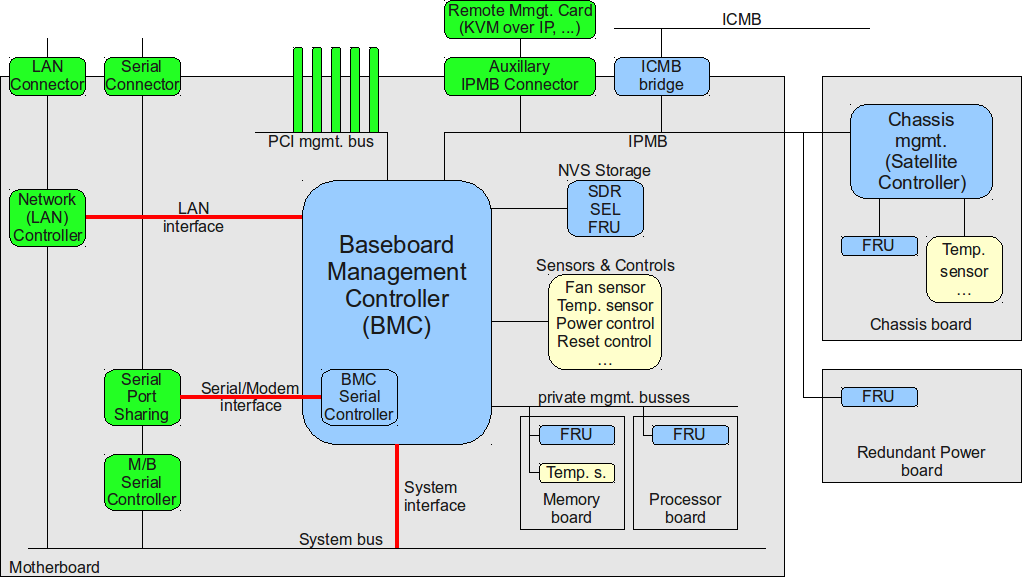
\includegraphics[width=0.95\textwidth]{swstk/ipmi-schem}
  \caption{IPMI结构框图}
  \label{fig:ipmi-schem}
\end{figure}

\textbf{Baseboard Management Controller (BMC)}\quad
微处理器BMC是整个IPMI架构的核心,它提供系统管理软件与硬件交互的接口,
这些硬件通过IPMB与ICMB总线连接到BMC(见下文),
实现系统的监控、控制与日志记录。

\textbf{Intelligent Platform Management Bus (IPMB)}\quad
IPMI使用IPMB标准实现BMC控制功能的扩展,IPMB是一个基于$I^2C$的串行总线,
用于节点内连接实现BMC扩展的卫星控制器(satellite controller),
并提供它们之间的通信功能。

\textbf{Intelligent Chassis Management Bus (ICMB)}\quad
在具有多BMC的服务器上,ICMB为这些BMC提供统一的通信与控制接口,实现统一管理。

%PRM在其基础上通过控制平面与控制平面网络,将资源管理功能也增加到其中,PRM具体架构在第\ref{chap:prm:arch}节将进行详细介绍。

\section{PARD软件栈架构}

\subsection{PRM管理模块}
\label{chap:prm:arch}

PARD使用带外管理的方式实现硬件资源的管理,
资源管理相关的软件栈运行在独立的平台资源管理模块(PRM)上。
如图\ref{fig:pard-swstk-arch}所示,
PRM是一个嵌入式的SoC系统,其中集成了处理器、内存、flash存储、以太网接口等模块;
与IPMI/BMC模块使用IPMB/ICMB总线连接其控制单元类似,
PRM通过控制平面网络(Control Plane Network,CPN)连接系统中所有的控制平面,
以实现节点内集中式的资源管理;
多台服务器的PRM模块共同连接到数据中心管理系统中,实现数据中心内统一资源管理。

\begin{figure}[tb]
  \centering
  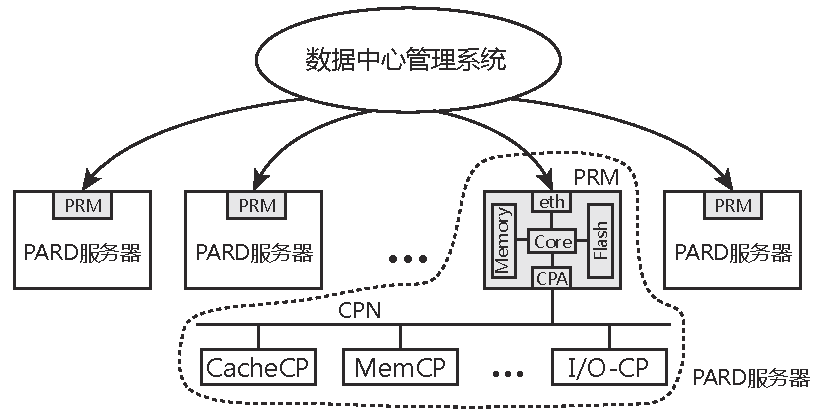
\includegraphics[width=0.8\textwidth]{swstk/pard-swstk-arch}
  \caption{PARD软件栈架构示意图}
  \label{fig:pard-swstk-arch}
\end{figure}


PRM上运行基于Linux操作系统的固件,使用分层的方式实现,如图\ref{fig:prm-swstk}所示,
从下到上依次是:1)控制平面驱动;2)控制平面抽象层;3)应用适配层。

控制平面驱动层提供对所有控制平面的访问功能,
它会在/dev目录下为每个连接到CPN上的控制平面创建对应的设备文件
(\emph{e.g.} /dev/cpa[0-9][0-9]*),
对这些设备文件的访问会被驱动转换为对16位的控制平面地址空间的访问,
通过第\ref{chap:hwresman}章所介绍的控制平面访问接口,
实现对控制表及数据平面的访问。

在控制平面驱动层的基础上,控制平面抽象层提供了更加友好的控制平面访问接口。
利用linux的sysfs\cite{patrick_mochel_sysfs_2005}机制,实现控制平面的抽象,
在/sys目录下为每个控制平面建立如图\ref{fig:prm-swstk}所示的目录结构
(\emph{e.g.} /sys/cpa/cpa[0-9][0-9]*),提供对控制平面的统一编程接口。
用户可以使用文件系统系统调用(如read/write/ioctl),
操作/dev目录下的设备文件实现控制平面编程,
也可以直接使用bash命令(如echo/cat等)操作/sys目录下的文件实现对控制平面编程。
直接操作/sys中的文件是更为推荐的方式。
基于sysfs的控制平面抽象及其功能将在下节进行详细描述。

应用适配层提供PARD体系结构在不同使用场景中的接口,
本文PARD原型系统实现了本地逻辑域和Mesos Slave 2个接口,
分别用于单节点资源管理与数据中心多节点资源管理。

当服务器加电后PRM首先启动,由控制平面驱动枚举控制平面网络,识别系统中的控制平面;
然后通过控制平面获取服务器的硬件资源信息,并建立sysfs下的控制平面抽象;
后续管理员或数据中心管理系统通过应用适配层与PRM交互,
将PARD服务器配置为多个逻辑域,运行用户的应用。

%管理员可以为每个应用设定其监控条件,当某一硬件控制平面发现监控条件满足时,
%则通过PRM通知上层管理架构,管理员可以通过PRM对不同应用的硬件资源使用进行管理。
%本节后续将从逻辑域的创建、监控条件设定、参数调整3个方面介绍PARD服务器操作。

\begin{figure}[tb]
  \centering
  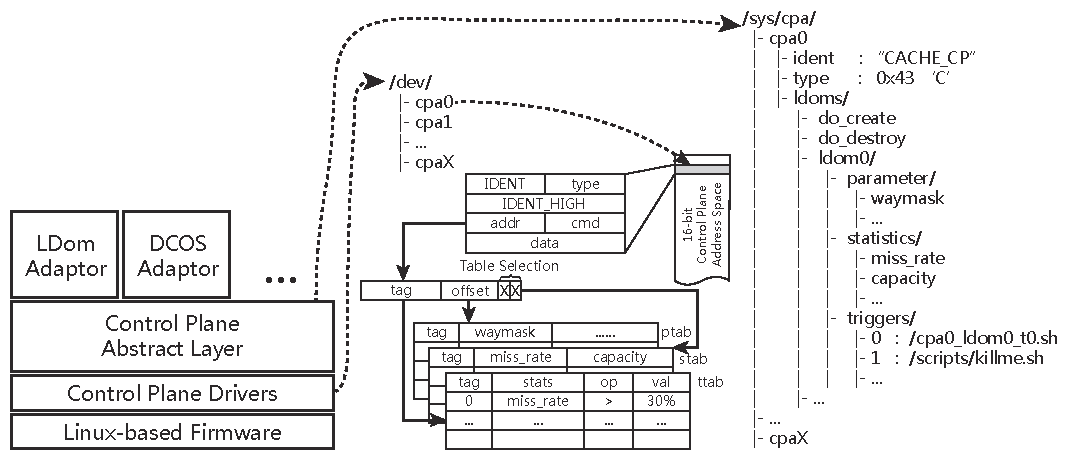
\includegraphics[width=\textwidth]{swstk/prm-swstk.pdf}
  \caption[PRM软件栈示意图]{PRM软件栈示意图}
  \label{fig:prm-swstk}
\end{figure}


\subsection{控制平面接口}
\label{chap:prm:arch:cpabs}

PRM利用linux的sysfs机制为用户(数据中心管理系统)提供控制平面的统一访问接口,
如图\ref{fig:prm-swstk}所示。

在/sys/cpa目录下,每个控制平面被表示为树型目录结构,
在每个目录下都会包含控制平面的基本信息,
如标识ident、类型type,
本文实现的PARD原型系统支持的控制平面类型包括:
Core(``P'')、Cache(``C'')、内存控制器(``M'')和I/O Bridge(``B'')。
在控制平面的目录下还包含ldoms目录,
其中包含2个用于逻辑域控制的文件``do\_create''和``do\_destroy'',
分别用于创建和销毁逻辑域;
ldoms目录下的每个子目录代表该控制平面上当前存在的逻辑域。
向do\_create文件写入16位逻辑域编号即可在当前控制平面中创建该逻辑域,
例如使用如下命令即可在cpa0控制平面下创建逻辑域LDom\#4:
\begin{verse}
\textit{echo} 4 \textit{> /sys/cpa/cpa}0\textit{/ldoms/do\_create}
\end{verse}
与之相对,向do\_destroy文件写入16位逻辑域编号则会销毁当前控制平面中指定的逻辑域,
使用如下命令,即可将刚刚创建的逻辑域LDom\#4销毁:
\begin{verse}
\textit{echo} 4 \textit{> /sys/cpa/cpa}0\textit{/ldoms/do\_destroy}
\end{verse}

每当逻辑域被创建后,
其所在控制平面的ldoms目录下都会创建1个与逻辑域同名的子目录
(\emph{e.g.} ldom[0-9][0-9]*),
例如上文创建逻辑域LDom\#4的命令同时会在``/sys/cpa/cpa0/ldoms''
目录下创建名为ldom4的逻辑域目录。
该目录下包含parameters、statistics和triggers 3个子目录,
分别对应于控制平面内的3个控制表。
其中parameters和statistics子目录下的文件与其控制表项一一对应,
以图\ref{fig:prm-swstk}中Cacge控制平面cpa0为例,
其参数表的参数way\_mask、以及状态表的miss\_rate和capacity都有相应的sysfs文件。
triggers目录与另外2个目录略有不同,该目录下为每个有效的触发表项建立对应的文件,
通过这个文件能够设置其触发条件满足时所执行的动作,
例如命令:
\begin{verse}
\textit{echo /scripts/some-scripts.sh > /sys/cpa/cpa}0
\textit{/ldoms/ldom}0
\textit{/triggers/}0
\end{verse}
会设置0号触发条件所执行的动作。
在实际情况下,不仅可以使用shell脚本作为触发动作,
在PRM上支持的任意语言的脚本、甚至可执行的ELF文件都可以作为触发动作,
通过sysfs安装到对应的触发条件上。
当前的原型系统实现,无法使用sysfs接口创建新的触发条件,
只能访问/dev目录下的设备文件,直接操作触发表(ttab)来创建触发条件,
sysfs接口只提供对触发动作的修改功能。


\section{节点内资源管理}

数据中心管理系统所提供的功能需要节点内提供相应支持,
本节介绍PRM软件栈如何实现这些支持,具体包括
逻辑域管理、资源隔离和性能监控3个方面。

\subsection{逻辑域管理}

PARD服务器使用逻辑域抽象为用户提供服务,
每个逻辑域都是PARD服务器硬件资源的子集,可直接在其中运行操作系统。
不同的逻辑逻辑域独占部分资源,如处理器核、内存、I/O设备;
另一些硬件资源在不同逻辑域中共享,如处理器末级缓存。
当PRM收到逻辑域的创建请求后,PRM首先确认当前服务器是否有足够的资源满足逻辑域的需求,
如果满足,则为其分配本地唯一的逻辑域标识,
之后在各个硬件资源的控制平面中为该逻辑域分配所需的资源。
例如,用户创建的逻辑域需要2个处理器核、2GB内存、1个硬盘和1个网卡,
PRM在确认本地资源充足后,为其分配逻辑域标识LDom\#1,后续的创建流程如下:

%%TODO: 增加sysfs相关的代码
\begin{enumerate}[leftmargin=2\parindent, nolistsep, label=\arabic*)]
  \item 查询处理器核的控制平面,找到2个空闲的处理器核,并向其标签寄存器写入LDom\#1,
        这2个处理器核后续发出的请求中将都包含该逻辑域标签。
  \item 在Cache控制平面中增加LDom\#1的控制表项,
        由于该用户在创建逻辑域时并没有对Cache指定特殊需求,
        因此为其分配默认的替换策略掩码,与其他用户共享Cache。
  \item PRM查询内存地址分配,找到空闲的2GB内存空间,
        在内存控制器控制平面中建立逻辑域LDom\#1的控制表项,
        将查询到的2GB空闲内存的地址写入控制表项,保存逻辑域与内存地址的关联,
        内存控制器在收到后续带有LDom\#1标签的访存请求后,会将查询地址映射信息,
        将来自不同逻辑域的访存地址映射到其对应的内存区域中。
  \item PRM为逻辑域分配磁盘和网卡,通过I/O控制平面将2个设备的标签寄存器设置为LDom\#1。
        这2个设备对内存的DMA请求中都包含该标签,保证其能够访问到逻辑域的内存地址空间;
        当前大部分的PCI-E设备都使用MSI方法产生中断,而MSI的本质是对特殊地址的访存请求,
        该请求中已经包含了逻辑域标签,
        因此中断请求能够被正确的发送到分配给该逻辑域的处理器核。
  \item PRM查询这2个设备在I/O总线上的物理地址以及所需的I/O地址空间长度,
        在逻辑域的地址空间中为这2个设备分配地址空间,
        通过I/O控制平面将分配的逻辑域地址空间与设备的物理地址映射记录到LDom\#1的控制表项。
\end{enumerate}

在资源分配完成后,PRM通过处理器控制平面,将2个处理器核复位,
之后选择1个处理器核作为Bootstrap Processor(BSP),令其开始执行BIOS代码,并启动操作系统。
%由于不同的逻辑域使用不同的标识,在整个计算机的数据通路中都能够根据该标识对逻辑域实现区分,
%实现逻辑域之间的资源隔离。

%用户的应用在运行时对硬件资源的需求会发生变化,PARD提供了运行时调整硬件资源分配的方法,
%允许用户根据需求在运行时对逻辑域的资源分配进行调整,以满足应用的需求。
%硬件资源包括可透明调整的资源,如Cache容量、访存带宽等;
%也包括需要操作系统支持的资源,如处理器核、内存容量、I/O设备。
%
%在创建逻辑域时,同时还可以指定其性能参数,如Cache替换策略掩码、访存调度优先级、
%I/O带宽等,各个硬件部分根据其控制平面中指定的性能参数实现对不同逻辑域的区分化服务。


\subsection{资源隔离}

由于没有相关的硬件支持,当前系统主要使用软件(如cgroup和hypervisor)进行资源隔离,
软件主要是通过调度的方式实现资源隔离,
通过调整不同应用的调度策略,实现资源隔离。

PARD提供了更为直接的资源隔离方案,
由于硬件已经通过控制平面参数表将其可调整的策略提供给上层软件,
并通过PRM的sysfs抽象将其暴露给用户。
因此在PARD系统上实现资源隔离,只需要通过sysfs接口对不同应用的资源占用进行调整即可。

以处理器末级缓存为例,
在使用默认参数创建逻辑域时,所有的逻辑域都共享处理器末级缓存资源,
如果这些应用中存在一些受缓存影响较大的关键应用时,
可以使用以下命令控制Cache控制平面,对缓存容量进行划分:

\begin{verse}
\textit{echo} 0x00FF \textit{>  /sys/cpa/cpa}0\textit{/ldoms/ldom}0\textit{/parameters/waymask} \\
\textit{echo} 0xFF00 \textit{>  /sys/cpa/cpa}0\textit{/ldoms/ldom}1\textit{/parameters/waymask} \\
\textit{echo} 0xFF00 \textit{>  /sys/cpa/cpa}0\textit{/ldoms/ldom}2\textit{/parameters/waymask} \\
\textit{echo} 0xFF00 \textit{>  /sys/cpa/cpa}0\textit{/ldoms/ldom}3\textit{/parameters/waymask} \\
\end{verse}

该命令设置LDom\#0独占8路缓存,另外3个逻辑域共享8路缓存,
通过缓存容量划分的方式实现资源隔离。


\subsection{性能监控与反馈}

按照性能监控的发起者,可将性能监控分为pull和push两类。
目前大多数系统都使用pull的方式获取硬件资源监控信息,
如处理器内常见的Performance Counter。
pull方式的性能监控需要用户主动参与,才能获取信息,实现实时性能监控开销很大。
PARD在控制平面上使用硬件实现资源监控,以硬件请求为粒度,将实时的状态信息更新到状态表中,
通过PRM软件栈的sysfs抽象,可以随时获取实时的状态信息。

PARD体系结构提供的``\emph{trigger$\Rightarrow$action}''机制,
可以用于实现实时的性能监控与反馈。
使用第\ref{chap:prm:arch:cpabs}节介绍的方法,为需要实时监控的状态设置触发条件,
并为其编写动作脚本,该脚本可以直接实现资源重新分配、或只是通知上层数据中心管理系统,
由其决定后续执行的动作。

%具体方法如下:
%Programming Methodology
%As mentioned in x3, we adopt a ``trigger$\Rightarrow$action'' programming
%methodology. Data center operators predefine a set of trigger)action
%rules for different priorities. Usually a trigger is based on performance
%metrics, \emph{e.g.}, ``MissRate>30\%''.
%Example 1 in Figure 6 demonstrates how to install a trigger)action
%rule. A data center operator uses the pardtrigger command to program
%the trigger condition ``MissRate>30\%'' for ``ldom=0'' (i.e.,
%DS-id=0) into the trigger table of the cache control plane (cpa0).
%The parameter ``action=0'' guides the command to create a leaf
%node ``0'' under ``.../cpa0/ldoms/ldom0/triggers''. Then the operator
%calls ``echo ...'' to install the action script ``/cpa0-ldom0-t0.sh''
%shown in Example 2.
%There are two programming approaches based on the device file
%tree. One is invoking system calls (open/read/write etc.) to open
%and manipulate a CPA file. For example, the pardtrigger command
%is written in C and invokes syscalls to install a trigger into the
%cache control plane. The advantage of this approach is very fast. A
%more convenient approach is leveraging bash commands to directly
%access these CPA files, as shown in Example 2.


\section{与数据中心结合}

% 云计算3种模型
云计算有3种模式:SaaS、PaaS、IaaS,%如图\ref{fig:cloud-usage-model}所示,
其区别在于用户需要管理的层次。
其中IaaS用户需要管理到OS层,如OpenStack;
PaaS用户只需要管理应用与数据,其他部分由数据中心管理,如Docker的使用模式;
SaaS是最底层,用户直接使用不同软件组合。
本章主要考查IaaS与PaaS两种模式。

%% -- removed by advisor
%%\begin{figure}[tb]
%%  \centering
%%  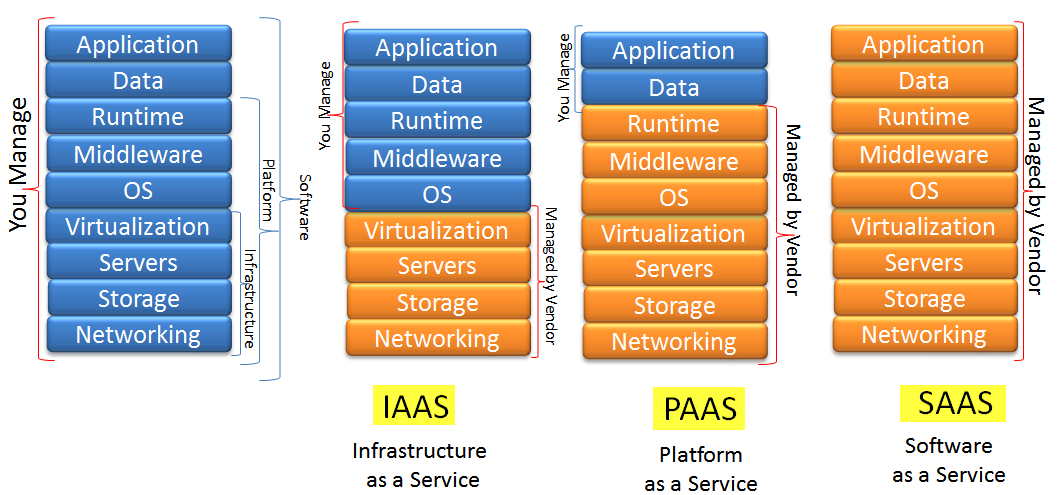
\includegraphics[width=0.8\textwidth]{swstk/cloud-usage-model}
%%  \caption{云计算3种使用模式对比:IaaS、PaaS与SaaS}
%%  \label{fig:cloud-usage-model}
%%\end{figure}

PARD提供的逻辑域抽象,能够很容易的实现IaaS模式,
因为逻辑域抽象与虚拟机抽象几乎完全相同,本文前几章的工作都是基于IaaS模式对PARD进行讨论。
但目前数据中心PaaS由于资源浪费较少,被越来越广泛的使用,
本节主要讨论如何在PARD平台上实现PaaS模式,同时将其集成到数据中心管理系统中,
这里将主要针对Mesos系统进行讨论。

\subsection{使用PARD体系结构实现PaaS}
% PARD如何实现PaaS
PARD实现PaaS的方式类似于
unikernel\cite{Unikernels:2013}或LibOS\cite{Porter:2011}的实现方式,
由用户提供应用与数据,并选择PARD软件栈所提供的运行时环境与库,
在运行时与PARD软件栈提供OS kernel组合,最终运行在PARD的逻辑域中。
具体流程如下,如图\ref{fig:pard-ldom-paas}:

1)用户提供需要执行的应用与数据,并选择所需的运行时环境和库;

2)将应用、数据、运行时环境打包为package,完成应用构建阶段;

3)系统根据用户选择的硬件资源配置创建逻辑域,将选择的内核与打包好的应用同时加载到逻辑域中;

4)将逻辑域在PARD服务器上启动。

\begin{figure}[tb]
  \centering
  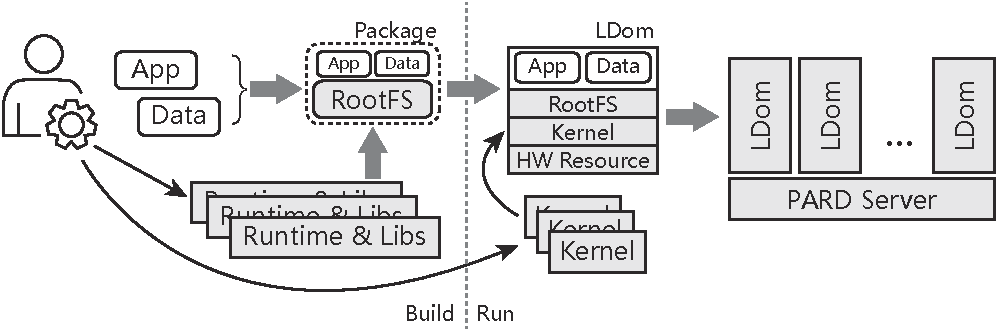
\includegraphics[width=\textwidth]{swstk/pard-ldom-paas}
  \caption{PARD体系结构实现PaaS模式}
  \label{fig:pard-ldom-paas}
\end{figure}

通过以上方式实现硬件支持的容器,该方法也可以在其它只提供IaaS抽象的场景中实现PaaS的功能。

\subsection{Mesos系统集成}
% Mesos如何管理资源

% PARD如何支持MesosExecutor
Mesos使用Containerizers组件在slave节点上实现任务的容器化,并负责任务容器的资源隔离、管理、以及状态收集。
当前版本(0.28.1)的Mesos实现了4种容器化方案,分别是:Composing Containerizer、Docker Containerizer、
Mesos Containerizer和External Containerizer,
其中Docker和Mesos Containerizer是最为常用的2种容器化方法,分别使用基于Docker引擎和cgroup实现任务的容器化。

在Mesos中运行任务分为3个阶段:
第1阶段是slave节点注册,将自身的资源汇报给master节点;
第2阶段由master将可用的资源列表发送给framework,由framework选择需要的资源,并调度任务给master;
第3阶段是slave接收master发送的任务,通过Containerizers执行该任务。

将PARD集成到Mesos系统中,需要对第1和3两个阶段进行修改。
在第1阶段,由于Mesos Slave属于带内的方式实现资源,
slave daemon运行在服务器操作系统之上,能够直接获得系统中的可用资源(如CPU、内存等);
而PARD的PRM使用带外的方式管理服务器资源,
直接使用原始的slave daemon获得的可用资源是PRM上的可用资源,
而不是服务器的可用资源。
因此,需要修改slave daemon,使其通过控制平面获取可用的服务器资源。

在第3阶段,需要为Mesos增加新的基于PARD逻辑域的容器化方法,
该容器化方法接收的任务是上节所述的package镜像,具体流程如下:

\begin{enumerate}[leftmargin=2\parindent, nolistsep, label=\arabic*)]
  \item master发送任务与资源信息到PARD服务的slave,该slave使用PARD的容器化方法执行任务;
  \item 在PRM中为该任务分配1个唯一的逻辑域编号,并根据资源信息在为该任务分配资源所在的控制平面上建立逻辑域;
  \item 根据资源分配信息,为逻辑域预留资源;
  \item 从master上获取任务的package;
  \item 通知PRM将该package加载到建立的逻辑域中,并启动该逻辑域。
\end{enumerate}

另一个需要考虑的问题的周期性的资源汇报,Mesos slave每隔一定的时间就会向master发送心跳信息,
同时其中还包含服务器当前资源使用情况。
与上文第1阶段的修改类似,需要修改slave的周期性资源状况收集模块,
使其通过控制平面获取当前资源的使用情况,
同时将控制平面中状态表的信息一同发送给master,为其提供更多的状态信息,
为实现更优化的任务调度策略提供数据基础。


%\subsection{PARD体系结构对数据中心管理系统的影响}
%% 对Mesos资源模型的影响
%%  -- PARD为Mesos增加了额外可控制的资源
%%  -- Mesos如何管理这些额外的资源
%%    -- 增加资源抽象属性:CPU/Mem => Cache/BW/QoS-Level/etc.
%%    -- 增加调度考查
%
%
\section{小结}

计算机软硬件需要协同工作,
PARD体系结构通过可编程的方式为上层软件提供了更多对硬件的控制能力,
这包括:应用区分、细粒度资源管理、应用区分的实时性能监控以及资源的反馈调节机制,
本章基于Linux sysfs机制设计了一种节点内资源管理抽象,为以上硬件特性实现了软件接口。
PARD提供的带外管理特性,使得系统管理与应用分离,实现单独控制;
其全硬件支持的虚拟化(逻辑域)特性,降低了软件开销与成本。
通过本章所提出的软件接口抽象,
可以很容易的将PARD体系结构到IaaS或PaaS模式的云计算平台下。
由于单节点可控制能力的增加,为数据中心管理系统提出了新的挑战,
%这主要由于可管理的资源种类增加、以及性能相关的调度因素。
如何在PARD这样的体系结构下设计出更灵活的作业调度与资源管理系统,
是未来软件设计的主要目标。

